\chapter{Travail réalisé}


\section{Aperçu général}
Voici la chronologie du travail réalisé en entreprise.\\
\ganttset{%
	calendar week text={%
		\pgfcalendarmonthshortname{\startmonth}~\startday%
	}%
}
\newganttlinktype{f-m}{
	\ganttsetstartanchor{on right=1}
	\ganttsetendanchor{on left=0}
	\draw[/pgfgantt/link]
	([xshift=-.2pt]\xLeft, \yUpper) --       % xshift to fit arrow
	node[pos=.5, /pgfgantt/link label node] {\ganttlinklabel} 
	(\xRight, \yLower);
}


%vgrid={*1{blue!30},
%	*6{black,dotted},
%	*1{red!30},
%	*2{black,dotted},
%	*1{blue!30},
%	*{34}{black,dotted},
%	*1{green!30},
%	*1{red!30},
%	*{10}{black,dotted},
%	*1{green!30}},
\setganttlinklabel{f-m}{}

\begin{ganttchart}[
	hgrid,
	vgrid,
	x unit=2.9mm,
	time slot format=isodate,
	inline,
	bar/.append style={fill=blue!37},
	group/.append style={draw=black, fill=black!50},
	milestone/.append style={fill=green, rounded corners=6pt,scale=2},
	milestone inline label node/.append style={right=1mm},
	]{2019-03-28}{2019-05-25}
	\gantttitlecalendar{year, month=name, week} \\
	\ganttgroup{Analyse des besoins}{2019-03-29}{2019-04-7}\\
	\ganttgroup{Réalisation technique}{2019-04-5}{2019-05-13}\\
	\ganttgroup{Maintenance}{2019-05-13}{2019-05-24} \\
	\ganttbar{OFBiz}{2019-04-01}{2019-04-11}\\
	\ganttbar[
	bar/.append style={ fill=red!50
	}]{REST}{2019-04-08}{2019-04-28} \\
	\ganttbar[
	bar/.append style={ fill=orange!50
	}]{Entitymaint}{2019-04-20}{2019-05-12} \\
	
	\ganttmilestone{Preuve de concept}{2019-05-12}] \\
	\ganttbar[
	bar/.append style={ fill=purple!40, dashed
	}]{Revue de code}{2019-05-13}{2019-05-23} \\
	\ganttlink{elem3}{elem4}
	\ganttlink{elem4}{elem5}
	\ganttlink[link type=f-m]{elem5}{elem6}
	\ganttlink[link type=dr]{elem4}{elem6}
	\ganttlink[link type=f-m]{elem6}{elem7}
\end{ganttchart}

\newpage









\section{Environnement}

\subsection{Installation de l'environnement}
Avant tout, mon intégration a commencé par l'installation du poste de travail suivi par une discussion sur le choix de distribution Linux \footnote{Une question qui a, apparemment, beaucoup d'importance.} , la configuration des outils utilisés par l'entreprise ainsi que par la mise en place des accès aux ressources internes \footnote{Contenaient, à mon avis, des information sensibles, mais cela s'explique par le principe de transparence \ref{activite} }



\subsection{Conventions}
\subsection{Formation développeur générale}
\subsection{Jira}
\subsection{Approfondissement de Git }
\subsection{Découverte de communauté libre Apache}

\newpage
\section{Prise en main d'OFBiz}

\subsection{Premier plugin}

\subsection{Projets existants et leur structure}
\subsubsection{Décathlon}
RFID et tout ça
\subsubsection{Dejbox}
Pierre et Antoine ont tout géré 

\subsection{Problématique vis-à-vis du développement}
What is "fonctionnel"

\newpage

\section{Analyse de l'existant}
\subsection{ControlServlet}
\subsection{Mécanisme de résolution des URI}
\subsection{Filtres}
Delegateur et Dispatcher


\newpage

\section{Analyse des besoins et attentes de la maîtrise d'ouvrage}
\subsection{Structure générale des application web}
Les enjeux, les problématiques les solutions, *COURS MAURIZIO*
\subsection{API en cours}
RPC
\subsection{Controleur}
<request-map>...
\subsection{Besoins d'évolution}
Avenir
*Discussion communautaire*
\subsection{Representational state transfer}
\subsubsection{Histoire}
Roy Fielding
\subsubsection{Principe}
*Détailles du cours de Maurizio: idempotence, navigabilité par hyperlink, 
notion de ressource etc.
\subsubsection{Avantages}
\subsubsection{Examples d'API du style REST}
API REST de Twitter, SoundCloud, Wiktionnaire,\\
les différences entre la définition de Roy Fielding et l'implémentation de ces dernières

\subsection{Implementations existantes}
\subsubsection{Camel}
\subsubsection{JAX-RS}
Tentative d'intégration ---\\
ServletJaxRS fonctionnelle\\
Particularités techniques (annotations) \\
Conflit politique car n'est pas dans le même esprit de l'existant.\\



\newpage

\section{Réalisations techniques}

\subsection{Librairie CXF}
Problèmatique avec les dépendances supplementaires: 
Tika contient déjà le CXF
\subsection{Choix vers URITemplate}
description de classe
\subsection{\textit{OverrideView()} et le conflit avec les URI segmentées}
\subsection{Choix d'intégration en parallèle avec le système existant }
\subsection{Nouveau contrôleur}
\subsubsection{Compromis pour les conflits d'URI}

\subsection{Modification de la partie "Administration: gestion des entités"  (entitymaint)  }
\subsubsection{Choix de la partie illustrative}
\subsubsection{PUT vs POST}
\subsubsection{Clés composées}
\subsubsection{Formulaires génériques }
Create update dans un même formulaire.
\subsection{Stateless}
\subsubsection{Les réalisation par la communauté}

Jaques Le Roux Token en gardant la session.
\subsection{RESTClient pour la communauté}
\subsubsection{Généralisation de code}
\subsubsection{Correction d'incohérences}



\iffalse
\section{Besoins fonctionnels}

Après une analyse des besoins fonctionnels du projet, nous avons défini deux sous catégories. D'un côté, les besoins [...], de l'autre, les besoins [...].

\subsection{Sous-partie 1}

Bla

\subsection{Sous-partie 2}

Bla

\newpage

\section{Besoins non-fonctionnels}

Comme précédemment, nous avons choisi de distinguer deux catégories pour les besoins non-fonctionnels. D'une part, nous avons les besoins non-fonctionnels pour les [...], et d'autre part ceux pour [...]. Nous avons aussi pris en compte les contraintes de développement, que nous détaillerons à la fin de cette partie.

\subsection{Sous-partie 1}

Bla\\

Aperçu du rendu souhaité :

\begin{figure}[!h]
\begin{center}
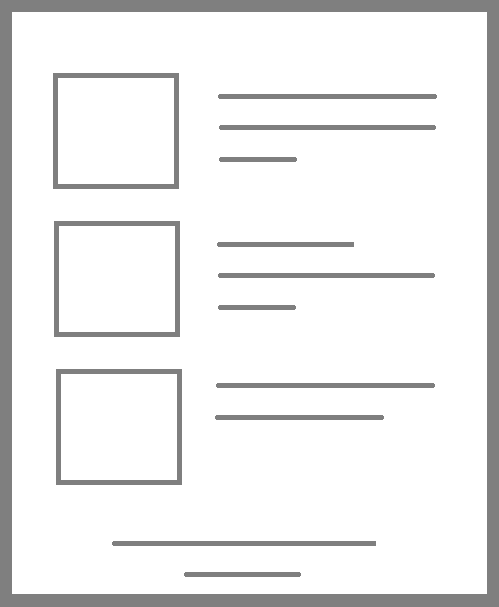
\includegraphics[height=10cm]{besoins/rendu}
\end{center}
\caption{Rendu attendu}
\end{figure}

\subsection{Sous-partie 2}

Bla

\newpage

\section{Développement}

Intro

\subsection{Tâches}

Bla\\


%tableau à taille fixée sur certaines colonnes (param sur la ligne \begin{tabularx}, voir wiki pour plus d'info sur la syntaxe
\begin{figure}[!h]
\begin{center}
\begin{tabularx}{17cm}{|c|p{6cm}|X|}
  \hline
  Priorité & Nom & Raison\\
  \hline
  1 & Tache 1 & Doit être vérifié en premier car sinon [...] \tabularnewline
  2 & Tache 2 & On doit pouvoir [...] \tabularnewline
  3 & Tache 3 & Comme les principales fonctionnalités permettant de tester sont opérationnelles, nous pouvons passer à cette tâche. \tabularnewline
  4 & Tache 4 & Parce que [...] \tabularnewline
  5 & Tache 5 & La tache 5 fait partie des principales [...]. \tabularnewline
  6 & Tache 6 & Dernière fonctionnalité essentielle à mettre en place. \tabularnewline
  7 & Tache 7 & Non-essentiel, mais apporterait un plus au projet. \tabularnewline
  8 & Tache 8 & Non-essentiel, mais apporterait un plus au projet. \tabularnewline
  \hline
\end{tabularx}
\end{center}
\caption{Tableau récapitulatif des tâches}
\end{figure}

\subsection{Tests}

Bla\\

\begin{figure}[!h]
\begin{center}
\begin{tabularx}{17cm}{|p{6cm}|X|}
  \hline
  Fonctionnalité & Test\\
  \hline
  Fonction 1 & Quand [...], vérifier [...]. \tabularnewline
  & Et quand [...], vérifier [...]. \tabularnewline
  Fonction 2 & Vérifier [...]. \tabularnewline
  Fonction 3 & Vérifier [...]. \tabularnewline
  Fonction 4 & Avoir [...]. \tabularnewline
  Fonction 5 & Accéder à [...]. \tabularnewline
   & Vérifier que [...]. \tabularnewline
  Fonction 6 & Accéder à [...]. \tabularnewline
   & Et vérifier [...]. \tabularnewline
  Fonction 7 & Installer [...]. \tabularnewline
   & Vérifier [...]. \tabularnewline
  Fonction 8 & Compter [...]. \tabularnewline
  \hline
\end{tabularx}
\end{center}
\caption{Tableau récapitulatif des tests}
\end{figure}
\fi